
L'intégration correspond au processus inverse de la dérivation. C'est un outil fondamental en mathématiques et en sciences, permettant de calculer des aires, des volumes, des moyennes, et de résoudre des équations différentielles.

\textit{Dans tout ce chapitre, $f$ et $g$ désignent deux fonctions continues sur un intervalle $[a, b]$.}

\section{Primitives et intégrales}

\subsection{Notion de primitive}

\begin{Def}\textbf{Primitive d'une fonction}

On dit qu'une fonction $F$ est une \textbf{primitive} de la fonction $f$ sur l'intervalle $[a ; b]$ si la dérivée de $F$ est égale à $f$.

C'est-à-dire qu'on a pour tout $x \in[a ; b]$ :
$$F^{\prime}(x)=f(x)$$    
\end{Def}

\begin{Rmq}
Si la fonction $F$ est une primitive de $f$, alors pour n'importe quel nombre réel $k$, la fonction $F+k$ est aussi une primitive de $f$.

Autrement dit, une primitive est définie \textbf{à une constante près}.
\end{Rmq}

\begin{Prop}\textbf{Ensemble des primitives}

Si $F$ est une primitive de $f$ sur $I$, alors l'ensemble de toutes les primitives de $f$ sur $I$ est :
$$\{F + C \mid C \in \mathbb{R}\}$$
\end{Prop}

\subsection{Tableau des primitives usuelles}

\renewcommand{\arraystretch}{2.3}
\begin{center}
\begin{tabular}{|c|c||c|c|}
\hline
\textbf{Fonction $f$} & \textbf{Primitive $F$} & \textbf{Fonction $f$} & \textbf{Primitive $F$} \\
\hline
$k$ (constante) & $kx + C$ & $u'(x) \cdot u^n(x)$, $n \neq -1$ & $\dfrac{u^{n+1}(x)}{n+1} + C$ \\
\hline
$x^n$, $n \neq -1$ & $\dfrac{x^{n+1}}{n+1} + C$ & $\dfrac{u'(x)}{u(x)}$ & $\ln |u(x)| + C$ \\
\hline
$\dfrac{1}{x}$ & $\ln |x| + C$ & $u'(x) e^{u(x)}$ & $e^{u(x)} + C$ \\
\hline
$e^x$ & $e^x + C$ & $\dfrac{u'(x)}{\sqrt{u(x)}}$ & $2\sqrt{u(x)} + C$ \\
\hline
$\dfrac{1}{x^n}$, $n \geq 2$ & $\dfrac{-1}{(n-1)x^{n-1}} + C$ & $\dfrac{u'(x)}{u^n(x)}$, $n \geq 2$ & $\dfrac{-1}{(n-1)u^{n-1}(x)} + C$ \\
\hline
$\cos x$ & $\sin x + C$ & $u'(x) \cos(u(x))$ & $\sin(u(x)) + C$ \\
\hline
$\sin x$ & $-\cos x + C$ & $u'(x) \sin(u(x))$ & $-\cos(u(x)) + C$ \\
\hline
$\dfrac{1}{\sqrt{x}}$ & $2\sqrt{x} + C$ & $\dfrac{1}{1+x^2}$ & $\arctan x + C$ \\
\hline
$\dfrac{1}{\cos^2 x}$ & $\tan x + C$ & $\dfrac{1}{\sqrt{1-x^2}}$ & $\arcsin x + C$ \\
\hline
\end{tabular}
\end{center}

\vspace{1em}\hrule\vspace{1em}

\exo[1]{\textbf{QCM - Primitives usuelles}}

Pour chaque fonction, indiquer la bonne primitive :

\begin{enumerate}
\item Une primitive de $f(x) = 4x^3 - 3x^2 + 2$ est :
\begin{multicols}{3}
\begin{enumerate}[label=\alph*.]
\item $12x^2 - 6x$
\item $x^4 - x^3 + 2x$
\item $x^4 - x^3 + 2x + 5$
\end{enumerate}
\end{multicols}

\item Une primitive de $f(x) = \dfrac{2x}{x^2+1}$ est :
\begin{multicols}{3}
\begin{enumerate}[label=\alph*.]
\item $\dfrac{1}{x^2+1}$
\item $\ln(x^2+1)$
\item $\arctan x$
\end{enumerate}
\end{multicols}

\item Une primitive de $f(x) = \cos(3x)$ est :
\begin{multicols}{3}
\begin{enumerate}[label=\alph*.]
\item $\sin(3x)$
\item $\dfrac{\sin(3x)}{3}$
\item $3\sin(3x)$
\end{enumerate}
\end{multicols}
\end{enumerate}

\vspace{1em}\hrule\vspace{1em}

\subsection{Intégrale définie}

\begin{Def}\textbf{Intégrale}

On appelle \textbf{intégrale de $f$ entre $a$ et $b$} et on note
$$\int_a^b f(x) \, dx$$
l'aire algébrique (en unités d'aire) délimitée par la courbe de $f$, l'axe des abscisses, et les droites verticales $x = a$ et $x = b$.
\end{Def}

\begin{figure}[h]
\centering
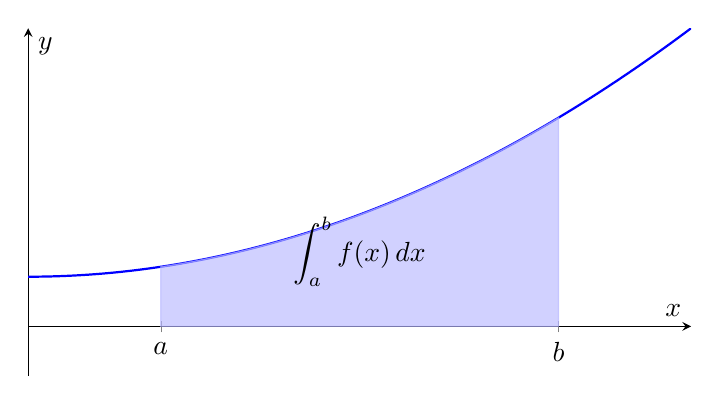
\begin{tikzpicture}
  \begin{axis}[
    axis lines = middle,
    xlabel = $x$,
    ylabel = {$y$},
    xmin=0, xmax=5,
    ymin=-1, ymax=6,
    xtick={1,4},
    xticklabels={$a$, $b$},
    ytick=\empty,
    domain=0:5,
    samples=100,
    width=10cm,
    height=6cm,
  ]
  \addplot[thick, blue, domain=0:5] {x^2/5 + 1};
  \addplot [domain=1:4, samples=100, blue!30, fill=blue!30, opacity=0.6]
  {x^2/5 + 1} \closedcycle;
  \node at (axis cs:2.5,1.5) {$\displaystyle \int_a^b f(x)\,dx$};
  \end{axis}
\end{tikzpicture}
\caption{Interprétation géométrique de l'intégrale}
\end{figure}

\begin{Rmq}
L'aire est dite \textbf{algébrique} car :
\begin{itemize}
\item Elle est comptée positivement lorsque $f(x) \geq 0$
\item Elle est comptée négativement lorsque $f(x) \leq 0$
\end{itemize}
\end{Rmq}

\subsection{Théorème fondamental de l'analyse}

\begin{Thm}\textbf{Théorème fondamental de l'analyse}

Soit $F$ une primitive de $f$ sur $[a,b]$. Alors :
$$\int_a^b f(x) \, dx = \big[F(x)\big]_a^b = F(b) - F(a)$$

La valeur de l'intégrale \textbf{ne dépend pas} du choix de la primitive.
\end{Thm}

\begin{Ex}
Calculer $\displaystyle\int_1^3 x \, dx$.

Une primitive de $f(x) = x$ est $F(x) = \dfrac{x^2}{2}$.

$\displaystyle\int_1^3 x \, dx = \left[\frac{x^2}{2}\right]_1^3 = \frac{9}{2} - \frac{1}{2} = 4$
\end{Ex}

\vspace{1em}\hrule\vspace{1em}

\exo[1]{\textbf{Calculs d'intégrales}}

Calculer les intégrales suivantes :

\begin{multicols}{3}
\begin{enumerate}
\item $\displaystyle\int_1^3 x \, dx$
\item $\displaystyle\int_{-2}^1 6x^2 \, dx$
\item $\displaystyle\int_0^{\ln 3} e^{2x} \, dx$
\item $\displaystyle\int_1^3 \frac{2x}{x^2+1} \, dx$
\item $\displaystyle\int_{\pi/4}^{\pi/3} \frac{\cos x}{\sin x} \, dx$
\item $\displaystyle\int_0^1 \frac{1}{1+x^2} \, dx$
\end{enumerate}
\end{multicols}

\vspace{1em}\hrule\vspace{1em}

\subsection{Propriétés de l'intégrale}

\begin{Prop}\textbf{Propriétés fondamentales}

\begin{enumerate}
\item \textbf{Intégrale sur un point :} $\displaystyle\int_a^a f(x) \, dx = 0$

\item \textbf{Changement de bornes :} $\displaystyle\int_a^b f(x) \, dx = -\int_b^a f(x) \, dx$

\item \textbf{Positivité :} Si $f \geq 0$ sur $[a,b]$, alors $\displaystyle\int_a^b f(x) \, dx \geq 0$

\item \textbf{Croissance :} Si $f \geq g$ sur $[a,b]$, alors $\displaystyle\int_a^b f(x) \, dx \geq \int_a^b g(x) \, dx$

\item \textbf{Inégalité triangulaire :} $\displaystyle\left|\int_a^b f(x) \, dx\right| \leq \int_a^b |f(x)| \, dx$

\item \textbf{Linéarité :} $\displaystyle\int_a^b \lambda f(x) + g(x) \, dx = \lambda \int_a^b f(x) \, dx + \int_a^b g(x) \, dx$

\item \textbf{Relation de Chasles :} Pour tout $c \in [a,b]$ :
$$\int_a^b f(x) \, dx = \int_a^c f(x) \, dx + \int_c^b f(x) \, dx$$
\end{enumerate}
\end{Prop}

\vspace{1em}\hrule\vspace{1em}

\section{Techniques d'intégration}

\subsection{Intégration par parties}

Le principe est d'exploiter la règle de Leibniz pour dériver un produit :
$$(uv)' = u'v + uv'$$

\begin{Thm}\textbf{Formule d'intégration par parties (IPP)}

Soient $f$ et $g$ deux fonctions dérivables de dérivées continues sur $[a,b]$. Alors :
$$\int_a^b f(x) g'(x) \, dx = \big[f(x) g(x)\big]_a^b - \int_a^b f'(x) g(x) \, dx$$
\end{Thm}

\begin{Rmq}
Toute la difficulté réside dans le choix de $f$ et de $g'$. Avec la pratique, ce choix devient plus naturel :
\begin{itemize}
\item On dérive ce qui se simplifie en dérivant ($\ln$, polynômes, $\arctan$...)
\item On primitive ce qui reste simple ($e^x$, $\sin$, $\cos$...)
\end{itemize}
\end{Rmq}

\begin{Ex}
Calculer $\displaystyle\int_0^1 x e^x \, dx$.

On pose $f(x) = x$ et $g'(x) = e^x$, donc $f'(x) = 1$ et $g(x) = e^x$.

$\displaystyle\int_0^1 x e^x \, dx = \big[x e^x\big]_0^1 - \int_0^1 e^x \, dx = e - \big[e^x\big]_0^1 = e - (e-1) = 1$
\end{Ex}

\begin{Ex}
Calculer $\displaystyle\int_1^e \ln x \, dx$.

On pose $f(x) = \ln x$ et $g'(x) = 1$, donc $f'(x) = \dfrac{1}{x}$ et $g(x) = x$.

$\displaystyle\int_1^e \ln x \, dx = \big[x \ln x\big]_1^e - \int_1^e x \cdot \frac{1}{x} \, dx = e \cdot 1 - 1 \cdot 0 - \big[x\big]_1^e = e - (e-1) = 1$
\end{Ex}

\begin{Ex}
Calculer $\displaystyle\int_0^{\pi/2} e^x \sin x \, dx$ (IPP double).

Posons $I = \displaystyle\int_0^{\pi/2} e^x \sin x \, dx$.

\vspace{1em}

\textbf{Première IPP :} $f = \sin x$, $g' = e^x$

$I = \big[e^x \sin x\big]_0^{\pi/2} - \int_0^{\pi/2} e^x \cos x \, dx = e^{\pi/2} - \int_0^{\pi/2} e^x \cos x \, dx$

\vspace{1em}

\textbf{Deuxième IPP :} $f = \cos x$, $g' = e^x$

$\displaystyle\int_0^{\pi/2} e^x \cos x \, dx = \big[e^x \cos x\big]_0^{\pi/2} + \int_0^{\pi/2} e^x \sin x \, dx = -1 + I$

Donc $I = e^{\pi/2} - (-1 + I) = e^{\pi/2} + 1 - I$

$2I = e^{\pi/2} + 1$, donc $I = \dfrac{e^{\pi/2} + 1}{2}$
\end{Ex}

\vspace{1em}\hrule\vspace{1em}

\exo[2]{\textbf{Intégration par parties}}

Calculer les intégrales suivantes :

\begin{multicols}{2}
\begin{enumerate}
\item $\displaystyle\int_0^{\pi/2} x \cos x \, dx$
\item $\displaystyle\int_0^1 x^2 e^{-x} \, dx$
\item $\displaystyle\int_1^e x \ln x \, dx$
\item $\displaystyle\int_0^1 \arctan x \, dx$
\item $\displaystyle\int_0^{\pi} x \sin x \, dx$
\item $\displaystyle\int_1^e (\ln x)^2 \, dx$
\end{enumerate}
\end{multicols}

\vspace{1em}\hrule\vspace{1em}

\subsection{Décomposition en éléments simples}

Il est toujours possible de déterminer l'expression d'une primitive d'une fraction de deux polynômes (fraction rationnelle).

\begin{Meth}\textbf{Principe de la décomposition}

L'objectif est de factoriser le dénominateur puis de découper la fraction en somme de fractions plus simples.

On considère $f$, $g$ et $h$ des polynômes. Pour calculer une primitive de $\dfrac{h}{fg}$, on cherche des polynômes $A$ et $B$ tels que :
$$\frac{h(x)}{f(x) g(x)} = \frac{A(x)}{f(x)} + \frac{B(x)}{g(x)}$$

En multipliant par $f(x)g(x)$ :
$$h(x) = A(x) g(x) + B(x) f(x)$$

On procède par identification des coefficients.
\end{Meth}

\begin{Ex}
Décomposer $\dfrac{1}{x^2-1}$ et calculer $\displaystyle\int_2^4 \frac{1}{x^2-1} \, dx$.

\textbf{Décomposition :} On cherche $a$ et $b$ tels que :
$$\frac{1}{(x-1)(x+1)} = \frac{a}{x-1} + \frac{b}{x+1}$$

Soit $1 = a(x+1) + b(x-1)$.

\begin{itemize}
\item Pour $x = 1$ : $1 = 2a$, donc $a = \dfrac{1}{2}$
\item Pour $x = -1$ : $1 = -2b$, donc $b = -\dfrac{1}{2}$
\end{itemize}

Donc $\dfrac{1}{x^2-1} = \dfrac{1}{2}\left(\dfrac{1}{x-1} - \dfrac{1}{x+1}\right)$

\textbf{Intégrale :}
$\displaystyle\int_2^4 \frac{1}{x^2-1} \, dx = \frac{1}{2}\left[\ln|x-1| - \ln|x+1|\right]_2^4 = \frac{1}{2}\left[\ln\frac{|x-1|}{|x+1|}\right]_2^4$

$= \dfrac{1}{2}\left(\ln\dfrac{3}{5} - \ln\dfrac{1}{3}\right) = \dfrac{1}{2}\ln\dfrac{9}{5}$
\end{Ex}

\vspace{1em}\hrule\vspace{1em}

\exo[2]{\textbf{Décomposition en éléments simples}}

\begin{enumerate}
\item Déterminer $a$ et $b$ tels que $\dfrac{x}{2x^2+9x+9} = \dfrac{a}{x+3} + \dfrac{b}{2x+3}$.

En déduire $\displaystyle\int_0^1 \frac{x}{2x^2+9x+9} \, dx$.

\item Déterminer $a$, $b$ et $c$ tels que $\dfrac{x-2}{(x^2+1)(2x+1)} = \dfrac{ax+b}{x^2+1} + \dfrac{c}{2x+1}$.

En déduire $\displaystyle\int_0^1 \frac{x-2}{(x^2+1)(2x+1)} \, dx$.

\item Calculer $\displaystyle\int_2^3 \frac{3x+1}{x^2-1} \, dx$.
\end{enumerate}

\vspace{1em}\hrule\vspace{1em}

\subsection{Changement de variable}

Vous avez déjà effectué des changements de variables pour résoudre des équations ou calculer des limites. C'est le même principe ici, combiné avec la formule de dérivation d'une composée de fonctions :
$$(f \circ g)' = (f' \circ g) \times g'$$

\begin{Thm}\textbf{Formule de changement de variable}

Soit $I$ un intervalle, soit $\varphi : [a,b] \to I$ continue dérivable et de dérivée continue. Alors :
$$\int_a^b f(\varphi(x)) \cdot \varphi'(x) \, dx = \int_{\varphi(a)}^{\varphi(b)} f(u) \, du$$

En posant $u = \varphi(x)$, ce qui implique $du = \varphi'(x) \, dx$.
\end{Thm}

\begin{Rmq}
La difficulté réside dans le choix de $\varphi$. Dans les cas les plus complexes, on précisera le changement de variable à effectuer.

\vspace{1em}

\textbf{Attention :} Ne pas oublier de changer les bornes !
\end{Rmq}

\begin{Ex}
Calculer $\displaystyle\int_0^1 \frac{e^x}{1+e^{2x}} \, dx$.

On pose $u = e^x$, donc $du = e^x \, dx$.

Bornes : $x = 0 \Rightarrow u = 1$ et $x = 1 \Rightarrow u = e$.

$\displaystyle\int_0^1 \frac{e^x}{1+e^{2x}} \, dx = \int_1^e \frac{1}{1+u^2} \, du = \big[\arctan u\big]_1^e = \arctan e - \frac{\pi}{4}$
\end{Ex}

\begin{Ex}
Calculer $\displaystyle\int_{-1}^1 \sqrt{1-x^2} \, dx$ en posant $x = \sin u$.

On a $dx = \cos u \, du$ et $\sqrt{1-x^2} = \sqrt{1-\sin^2 u} = |\cos u| = \cos u$ (car $u \in [-\frac{\pi}{2}, \frac{\pi}{2}]$).

Bornes : $x = -1 \Rightarrow u = -\frac{\pi}{2}$ et $x = 1 \Rightarrow u = \frac{\pi}{2}$.

$\displaystyle\int_{-1}^1 \sqrt{1-x^2} \, dx = \int_{-\pi/2}^{\pi/2} \cos^2 u \, du = \int_{-\pi/2}^{\pi/2} \frac{1+\cos(2u)}{2} \, du$

$= \dfrac{1}{2}\left[u + \dfrac{\sin(2u)}{2}\right]_{-\pi/2}^{\pi/2} = \dfrac{1}{2}\left(\dfrac{\pi}{2} + \dfrac{\pi}{2}\right) = \dfrac{\pi}{2}$

On retrouve bien l'aire d'un demi-disque de rayon 1.
\end{Ex}

\vspace{1em}\hrule\vspace{1em}

\exo[2]{\textbf{Changement de variable}}

\begin{enumerate}
\item En posant $u = \sqrt{x+1}$, calculer $\displaystyle\int_0^3 \frac{x}{\sqrt{x+1}} \, dx$

\item En posant $u = \ln x$, calculer $\displaystyle\int_1^e \frac{\ln x}{x} \, dx$

\item En posant $u = \tan x$, calculer $\displaystyle\int_0^{\pi/4} \frac{1}{\cos^2 x (1+\tan^2 x)} \, dx$

\item Calculer $\displaystyle\int_0^1 \frac{x}{\sqrt{1+x^2}} \, dx$
\end{enumerate}

\vspace{1em}\hrule\vspace{1em}

\subsection{Le cas de l'arctangente}

C'est un cas particulier important à connaître :

\begin{Prop}\textbf{Primitives avec arctangente}

$$\int \frac{1}{1+x^2} \, dx = \arctan x + C$$

Via un changement de variable, on peut généraliser :
$$\int \frac{1}{a^2+x^2} \, dx = \frac{1}{a} \arctan\left(\frac{x}{a}\right) + C$$
pour tout $a$ réel non nul.
\end{Prop}

\begin{Ex}
Calculer $\displaystyle\int_0^{1/\sqrt{2}} \frac{1}{2x^2+1} \, dx$.

On écrit $\dfrac{1}{2x^2+1} = \dfrac{1}{(\sqrt{2}x)^2+1}$.

Posons $u = \sqrt{2}x$, donc $du = \sqrt{2} \, dx$.

$\displaystyle\int_0^{1/\sqrt{2}} \frac{1}{2x^2+1} \, dx = \frac{1}{\sqrt{2}}\int_0^1 \frac{1}{1+u^2} \, du = \frac{1}{\sqrt{2}}\left[\arctan u\right]_0^1 = \frac{\pi}{4\sqrt{2}} = \frac{\pi\sqrt{2}}{8}$
\end{Ex}

\begin{Ex}
Calculer $\displaystyle\int_0^1 \frac{1}{x^2-x+1} \, dx$.

On complète le carré : $x^2 - x + 1 = \left(x - \dfrac{1}{2}\right)^2 + \dfrac{3}{4}$

Posons $u = x - \dfrac{1}{2}$, donc $du = dx$.

$\displaystyle\int_0^1 \frac{1}{x^2-x+1} \, dx = \int_{-1/2}^{1/2} \frac{1}{u^2 + 3/4} \, du = \frac{1}{3/4}\int_{-1/2}^{1/2} \frac{1}{1 + (2u/\sqrt{3})^2} \, du$

$= \dfrac{4}{3} \cdot \dfrac{\sqrt{3}}{2}\left[\arctan\dfrac{2u}{\sqrt{3}}\right]_{-1/2}^{1/2} = \dfrac{2\sqrt{3}}{3}\left(\arctan\dfrac{1}{\sqrt{3}} - \arctan\dfrac{-1}{\sqrt{3}}\right) = \dfrac{2\sqrt{3}}{3} \cdot \dfrac{\pi}{3} = \dfrac{2\pi\sqrt{3}}{9}$
\end{Ex}

\vspace{1em}\hrule\vspace{1em}

\section{Exercices récapitulatifs}

\exo[1]{\textbf{Calculs de primitives}}

Déterminer une primitive des fonctions suivantes :

\begin{multicols}{3}
\begin{enumerate}
\item $f(x) = 3x + 1$
\item $f(x) = 3x^2 - x + 1$
\item $f(x) = \dfrac{1}{x} + 2$
\item $f(x) = e^x + 1$
\item $f(x) = \dfrac{3}{x+1} - e^{2x+1}$
\item $f(t) = t \cdot e^{t^2+1}$
\item $f(t) = \dfrac{e^t}{e^t+1}$
\item $f(t) = \dfrac{e^{2t}-1}{e^t}$
\item $f(t) = \dfrac{t^2-t}{t^3}$
\item $f(t) = \dfrac{3t-2}{2t^2-5t-3}$
\end{enumerate}
\end{multicols}

\textit{Pour la dernière, on pourra remarquer que $2t^2 - 5t - 3 = (t-3)(2t+1)$.}

\vspace{1em}\hrule\vspace{1em}

\exo[2]{\textbf{Calculs d'intégrales variés}}

Calculer les intégrales suivantes :

\begin{multicols}{2}
\begin{enumerate}
\item $\displaystyle\int_0^1 \ln(x+1) \, dx$ \quad (IPP)
\item $\displaystyle\int_1^{e^\pi} \sin(\ln x) \, dx$ \quad (IPP)
\item $\displaystyle\int_0^{\pi/2} x^2 \cos x \, dx$ \quad (IPP)
\item $\displaystyle\int_0^{\pi/2} \frac{\cos x}{1+\sin x} \, dx$
\item $\displaystyle\int_0^1 e^{\sqrt{t}} \, dt$
\item $\displaystyle\int_1^e \frac{1}{x\sqrt{\ln x + 1}} \, dx$ \quad ($u = \ln x$)
\end{enumerate}
\end{multicols}

\vspace{1em}\hrule\vspace{1em}

\exo[3]{\textbf{Problème - Un logo}}

On s'intéresse au logo symétrique ci-dessous :

La feuille gauche du logo correspond à la partie grisée du plan délimitée par les fonctions :
$$f(x) = \frac{0{,}2}{x} \quad \text{et} \quad g(x) = -x^2 + 0{,}2x + 1$$

L'unité choisie sur chacun des axes est de 2,5 cm.

\begin{enumerate}
\item Déterminer les abscisses des points d'intersection des courbes.
\item Calculer l'aire de la feuille gauche.
\item Calculer l'aire totale du logo en $cm^2$.
\end{enumerate}

\vspace{1em}\hrule\vspace{1em}

\exo[3]{\textbf{Problème - Hangar à peindre}}

Un architecte veut établir les plans d'un hangar pour ballon dirigeable. La façade avant est symétrique par rapport au segment vertical $[OS]$ et $OH = 30$ m.

L'arc $\widehat{SA}$ de la façade correspond à une partie de la courbe représentative de la fonction définie sur $[0, 60]$ par :
$$f(x) = 80 - 20e^{0{,}025x}$$

Le cahier des charges impose :
\begin{itemize}
\item $OS = 60$ m
\item $HK > 35$ m
\item $f$ strictement décroissante sur $[0, 60]$
\item $OA \leq 60$ m
\end{itemize}

\begin{enumerate}
\item Montrer que $f$ vérifie les conditions du cahier des charges.
\item On souhaite peindre la surface extérieure de la façade avant. La peinture utilisée est vendue en bidons de 68 litres avec un pouvoir couvrant de $0,2 m^2$ par litre. Combien de bidons sont nécessaires ?
\end{enumerate}

\vspace{1em}\hrule\vspace{1em}

\exo[3]{\textbf{Problème - Une cuve de fioul}}

On souhaite connaître le volume restant dans une cuve de fioul cylindrique horizontale de rayon 1 m.

On note $S(y)$ la surface rectangulaire horizontale de fioul dans la cuve (fonction de l'ordonnée $y$ qui varie entre $-1$ et $1$).

Le volume $V$ de fioul restant quand le niveau est à l'ordonnée $y$ vaut :
$$V(y) = \int_{-1}^y S(t) \, dt$$

\begin{enumerate}
\item Exprimer $S(y)$ en fonction de $y$.
\item Montrer que $\dfrac{t^2}{\sqrt{1-t^2}} = -\sqrt{1-t^2} + \dfrac{1}{\sqrt{1-t^2}}$.
\item En déduire le volume de fioul restant en fonction de $y$.
\item Calculer le volume total de la cuve.
\end{enumerate}

\vspace{1em}\hrule\vspace{1em}

\exo[3]{\textbf{Problème - Un prélèvement}}

On prélève via un tuyau cylindrique de l'eau dans la réserve d'eau de pluie de l'ESTP de 10 000 litres. Le débit d'eau, mesuré en litres par minute, varie en fonction du temps $t$ en minutes selon la formule :
$$D(t) = \frac{K}{(t+1)(t+2)}$$

Pour un prélèvement qui dure $x$ minutes, le volume prélevé est :
$$V(x) = \int_0^x D(t) \, dt$$

\begin{enumerate}
\item Décomposer $\dfrac{1}{(t+1)(t+2)}$ en éléments simples.
\item En déduire l'expression de $V(x)$.
\item Le prélèvement a duré 10 minutes et on a prélevé 2000 litres. Déterminer la constante $K$.
\item Combien de litres d'eau reste-t-il dans la réserve ?
\end{enumerate}

